\documentclass{article}
\usepackage{tikz}
\usetikzlibrary{arrows}

\tikzset{
  treenode/.style = {align=center, inner sep=0pt, text centered,
    font=\sffamily},
  arn_n/.style = {treenode, circle, white, draw=black,
    fill=black, text width=1.5em},% arbre rouge noir, noeud noir
  arn_l/.style = {treenode, circle, black, draw=black, 
    text width=1.5em},% arbre rouge noir, noeud rouge
}

\begin{document}
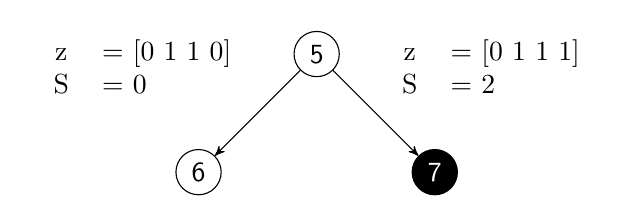
\begin{tikzpicture}[->,>=stealth',level/.style={sibling distance = 3cm/#1,
  level distance = 1.5cm}] 
\node [arn_l] {5}
        child{ node [arn_l] {6} 
    edge from parent node[above left] {\begin{tabular}{c l} z & = [0 1 1 0] \\ S & = 0 \end{tabular}} }
        child{ node [arn_n] {7}
    edge from parent node[above right] {\begin{tabular}{c l} z & = [0 1 1 1] \\ S & = 2 \end{tabular}} } 
    ;       
\end{tikzpicture}
\end{document}